\section{The Backpropagation algorithm}

\definecolor{darkgreen}{rgb}{0,0.6,0}
\definecolor{darkcyan}{rgb}{0,0.5,0.5}
\definecolor{darkyellow}{rgb}{0.5,0.5,0}
\definecolor{mangenta}{rgb}{1,0,1}

\begin{frame}\frametitle{\secname}

The Backpropagation algorithm is a method for computing gradients by using the chain rule efficiently.
\mode<article>{\eqref{eq:gradient_terms} shows us how the gradient breaks down into (1) an error term and (2) a term dependent on the type of model chosen. Specifically:
}	
\begin{equation}
	\textcolor{orange}{	\frac{\partial y(\vec{x}; \vec{w})}{
			\partial \mathrm{w}_{ij}^{v'v}}}
    \label{eq:model_term}
\end{equation}
    
The Backpropagation algorithm handles the computation of the term in \eqref{eq:model_term} for neural networks such as the one depicted in \figref{fig:example_mlp}.

\end{frame}

% -----------------------------------------------------------------------------
\begin{frame} \frametitle{Gradients in neural networks}
    
    \mode<article>{
    The Backpropagation algorithm is not tied to any specific neural architecture. We will therefore attempt to formulate how it works in the general sense.\\
    
    Let $w^{v'v}_{ij}$ be the weight connecting neuron $j$ in layer $v$ to neuron $i$ in layer $v'$, In order to compute $\frac{\partial y(\vec{x}; \vec{w})}{
			\partial \mathrm{w}_{ij}^{v'v}}$ we need to identify the following:
    \begin{itemize}
        \item $P(v, j)$: the set of immediate parent nodes feeding input into neuron $(v, j)$,
        \item $C(v', i)$: the set of immediate children nodes which neuron $(v', i)$ provides with input
    \end{itemize}
    }
    
    \begin{figure}[h]
    \centering   
    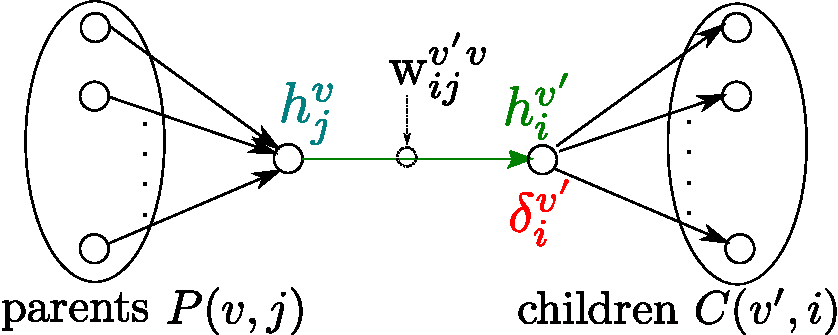
\includegraphics[height=3cm]{img/section1_fig20_mini_multicolor.pdf}
    \mode<article>{
    \caption{Nodes $(v,j)$ and $(v', i)$ are directly connected via the weight $w^{v'v}_{ij}$. The bias node for neuron $(v,j)$ is included in the set of its parent nodes.}
    }
    \label{fig:connection_ij}
    \end{figure}
    
    \mode<article>{
    $h^{v'}_{i}$ measures the total input arriving at neuron $i$ in layer $v'$.
    $h^{v'}_{i}$ is the weighted sum of this neuron's parent activations:
    }
    
    \mode<presentation>{\vspace{-5mm}
    }
    \begin{equation}
            {\color{darkgreen}h_i^{v'}} 
            := 
            \kern-2ex
            \sum_{(\mu,k) \in P(v',\,i)}
            \kern-2ex
            w_{ik}^{v'\mu}\; 
            f_k^\mu\big( {\color{teal} h_k^\mu} \big)   
            \label{eq:total_input_vi},
    \end{equation}
    
    \mode<article>{
    where $\mu$ and $k$ in \eqref{eq:total_input_vi} serve as indices for describing the position of each parent node in $P(v', i)$ in the network.
    }
    \mode<presentation>{\vspace{-5mm}
    }
    
    \pause 
    \question{How does $w_{ij}^{v'v}$ contribute to the error?
    \slidesonly{$\frac{\partial y(\vec{x}; \vec{w})}{\partial w_{ij}^{v'v}} = \ldots$
    }}\\
    
    \mode<article>{
    - The contribution is measured by applying the chain rule:
    }
    \mode<presentation>{\vspace{-9mm}
    }
    
    \begin{eqnarray}
        \frac{\partial y(\vec{x}; \vec{w})}{\partial w_{ij}^{v'v}}
            = \underbrace{\frac{\partial y(\vec{x}; \vec{w})}
                {{\color{darkgreen}\partial h_i^{v'}}} }_{ 
                    \substack{\coloneqq\;{\color{red}\delta_i^{v'}} \\
                    \text{``local error''} \\
                    \text{at neuron} \\
                    (v', i)}
                }
              \cdot 
              \underbrace{\frac{{\color{darkgreen}\partial h_i^{v'}}}
                {\partial w_{ij}^{v'v}}}_{
                    \substack{=\;f_j^v({\color{teal} h_j^v}) \\
                    \text{activity} \\
                    \text{of neuron} \\
                    (v, j)}}
                \label{eq:input_output_terms}
    \end{eqnarray}
    
    \mode<article>{
    \eqref{eq:input_output_terms} breaks the contribution of  $w_{ij}^{v'v}$ to the neuron's output into two parts:
    \begin{enumerate}
     \item The contribution of $h^{v'}_{i}$ to the network's response $y(\vec x; \vec w)$. This is referred to as the ``local error'' at neuron $(v',i)$. The efficiency of the Backpropagation algorithm is based on how it computes the ``local error'' denoted by $\delta_i^{v'}$ for neuron $(v', i)$ and all other neurons in the network.
     \item The contribution of $h^{v'}_{i}$ due to one of its inputs, namely neuron $(v,j)$ which is weighted by $w_{ij}^{v'v}$. We already have everything to compute this term and that is by taking the definition of $h^{v'}_{i}$ in \eqref{eq:total_input_vi} and taking the derivative w.r.t. $w_{ij}^{v'v}$. 
     This should be straightforward, since only a single term in the sum depends on $w_{ij}^{v'v}$:
         \begin{equation}
            \frac{{\color{darkgreen}\partial h_i^{v'}}}
            {\partial w_{ij}^{v'v}}
            =  \frac{\partial}
            {\partial w_{ij}^{v'v}}
            \left(
            \sum_{(\mu,k) \in P(v',\,i)}
            \kern-3ex
            w_{ik}^{v'\mu}\; 
            f_k^\mu\big( {\color{teal} h_k^\mu} \big){}
            \right)
            = \underbrace{f_j^v({\color{teal} h_j^v})}_{
            \substack{
                    \text{activity} \\
                    \text{of neuron} \\
                    (v, j)
                    }}
        \end{equation}
    \end{enumerate}
    }
\end{frame}

\begin{frame}\frametitle{The Backpropagation algorithm}
    The Backpropagation algorithm is composed of two stages:
    \begin{enumerate}
     \item \textbf{forward propagation} (forward pass)
     \mode<article>{: Given some input $\vec x$ compute the activities of all neurons and the response of the network.}
     \item \textbf{backwards propagation} (backward pass)
     \mode<article>{: Given the response of the network. Recursively calculate the local errors starting with the output node and work your way backwards through the network.}
    \end{enumerate}
\end{frame}

\subsection{Forward and backwards propagation}

% -----------------------------------------------------------------------------
\begin{frame} \frametitle{The Backpropagation algorithm}
    \mode<presentation>{
	\only<1,2>{\placeimage{9.5}{1}{img/section1_fig20_mini_multicolor.pdf}{width=4.8cm}}
	\only<3->{\placeimage{9.5}{1}{img/section1_fig20_mini_back_multicolor.pdf}{width=4.8cm}}
    }
    \mode<presentation>{ \vspace{11mm} }
	\begin{enumerate}
		\item \textbf{forward propagation}: calculate activities 
				$f_i^{v'}({\color{darkgreen}h_i^{v'}})$
				{\small(parents $\rightarrow$ children)}
				$$	
					{
					%\color{darkgreen}
					h_j^0
					} 
						\;:=\; \mathrm{x}_j \,, 
					\quad 
					{\color{darkgreen}h_i^{v'}}
		   			\,= \kern-2ex\smallsum{(\mu,k) \in P(v',\,i)}{} \kern-2ex
	   			w_{ik}^{v'\mu}\;  f_k^\mu\big( {\color{teal} h_k^\mu} \big) \,,
					\quad
					y(\vec{x}; \vec{w})\,=\, f_1^L({\color{blue}h_1^L})
				$$\\\vspace{-2mm}
	\only<1>{	
		\mode<presentation>{
		\begin{center}
		\vspace{2mm}
		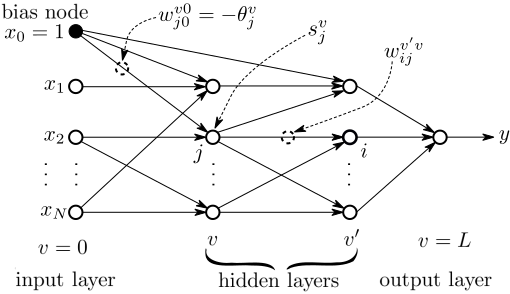
\includegraphics[height=4cm]{img/section1_fig14}
		\end{center}
		}
	}
	\only<2>{	
		\mode<presentation>{
		\begin{center}
		\vspace{2mm}
		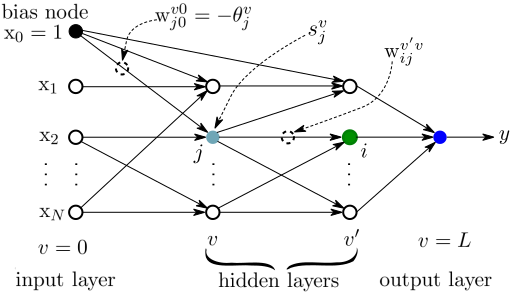
\includegraphics[height=4cm]{img/section1_fig14_fwd}
		\end{center}
		}
	}
	\only<3->{
		\item \textbf{backpropagation}: calculate ``local errors'' 
				$\color{red}\delta_i^{v'}$
				{\small(children $\rightarrow$ parents)}
				\vspace{-1mm}
				%~ \begin{eqnarray*} 
				%~ \end{eqnarray*}
				\begin{eqnarray} 
				{\color{red} \delta_1^L}
				&=& \frac{\partial y(\vec{x}; \vec{w})} {{\color{blue}\partial h_1^{L}}}
					= [f_1^{L}]'({\color{blue} h_1^{L}})
							%\;\;\text{for}\;v'=L
							\\
					{\color{red}\delta_i^{v'}} 
					\only<3>{
						&=&  \frac{\partial y(\vec x; \vec w)}{\color{darkgreen}\partial h^{v'}_{i}}
						\qquad \text{``local error'' at neuron }(v', i)
                        \label{eq:delta_step1}\\
						}
					\only<4->{
						&=&  \kern-3ex\sum\limits_{(v''\hspace{-1mm},\,k) \in C(v',\,i)}{
						\underbrace{
							\smallfrac{\partial y(\vec{x}; \vec{w})}
								{{\color{blue}\partial  h_k^{v''}}}
							}_{{\color{red}\delta_k^{v''}}} 
						\;\kern1.5ex\cdot \kern-2.5ex\;
						\underbrace{\smallfrac
								{{\color{blue}\partial h_k^{v''}} }
								{{\color{darkgreen}\partial h_i^{v'}}}
							}_{{w}_{ki}^{v''v'} \kern-.5ex\cdot\kern.5ex
								[f_i^{v'}]'({\color{darkgreen}h_i^{v'}}) }}
                            \label{eq:delta_step2}
                                \notesonly{\\&=&  \kern-3ex\sum\limits_{(v''\hspace{-1mm},\,k) \in C(v',\,i)}{
						{\kern-2ex {\color{red}\delta_k^{v''}}}
                        \cdot\,
						{{w}_{ki}^{v''v'} \kern-.5ex\kern.5ex
								[f_i^{v'}]'({\color{darkgreen}h_i^{v'}}) }}}
                                \notesonly{\\ \kern-3ex&=&\;\;\; }%\,,
                                \slidesonly{\kern-3ex=\;\;\; }%\underbrace{
							[f_i^{v'}]'({\color{darkgreen}h_i^{v'}}) 
							\kern-3ex\sum_{(v''\hspace{-1mm},\,k) \in C(v',\,i)}\kern-3ex
							{\color{red}\delta_k^{v''}} 
							{w}_{ki}^{v'' v'} 
						}
						%}_{{\color{red} \delta_i^L}\;=\;
						%	[f_i^{L}]'({\color{darkgreen} h_i^{L}})
						%	\;\;\text{for}\;v'=L}
				\end{eqnarray}
		}
		\only<5->{
		\vspace{-1mm}
		\item[] \textbf {weight update}: using activities and local errors
        \begin{equation}
				\mathrm{w}_{ij}^{v'v}
				\quad \leftarrow \quad 
				{w}_{ij}^{v'v} - \eta \cdot
				\smallfrac{\partial e}{\partial{w}_{ij}^{v'v}}
				\quad=\quad {w}_{ij}^{v'v} - \eta \cdot
				\smallfrac{\partial e}{\partial y(\vec{x}; \vec{w})} \cdot
				\only<5>{
				\smallfrac{\partial y(\vec{x}; \vec{w})}{\partial{w}_{ij}^{v'v}}\hspace{8.5mm}
				}
                \slidesonly{
				\only<6>{
				{\color{red} \delta_i^{v'}} \kern-.5ex\cdot
			   			f_j^v( {\color{darkgreen}h_j^v} )
			   	}}
        \end{equation}
        \notesonly{
        \begin{equation}
				\mathrm{w}_{ij}^{v'v}
				\quad \leftarrow \quad 
                {w}_{ij}^{v'v} - \eta \cdot
				\smallfrac{\partial e}{\partial y(\vec{x}; \vec{w})} \cdot
				{
				{\color{red} \delta_i^{v'}} \kern-.5ex\cdot
			   			f_j^v( {\color{darkgreen}h_j^v} )
			   	}
        \end{equation}
        }
			}
	\end{enumerate}
	%{\scriptsize
	%Computational complexity: $O(n)$, $n$: number of weights \& thresholds}
    
\end{frame}

\mode<article>{
    To understand how the ``local error'' at neuron $(v',i)$ goes from its definition in \eqref{eq:delta_step1} to \eqref{eq:delta_step2}, one needs to look at the propagation from $(v',i)$ forwards to all its immediate children nodes in $C(v', i)$. Let $(v'', k)$ describe a neuron positioned deeper in the network and connected to $(v',i)$, making it one of its children and, in turn, making $(v',i)$ one of the parents of $(v'', k)$.\\
    Analogous to how we compute in ${\color{darkgreen}h_i^{v'}}$ in \eqref{eq:total_input_vi}:
    
    \begin{align}
            {\color{blue}h_k^{v''}} 
            :=& 
            \kern-2ex
            \sum_{(\mu,\,l) \in P(v'',\,k)}
            \kern-2ex
            w_{kl}^{v''\mu}\; 
            f_l^\mu\big( {h_l^\mu} \big)   
            \label{eq:total_input_vddk}\\
            =&\; \ldots \,+\,{}
            w_{ki}^{v''v'}\; 
            f_i^{v'}\big( {\color{darkgreen}h_i^{v'}})
            \,+\, \ldots
    \end{align}
    
    Since only one term in this sum depends on ${\color{darkgreen} h_i^{v'}}$:
    \begin{align}
    \frac{{\color{blue}\partial h_k^{v''}} }{{\color{darkgreen}\partial h_i^{v'}}}
    \;&= \;
    \frac{\partial}{\color{darkgreen}\partial h_i^{v'}}
    \left(
    w_{ki}^{v''v'}\; 
            f_i^{v'}\big( {\color{darkgreen}h_i^{v'}})
    \right)\\
    \;&= \; w_{ki}^{v''v'} \,
    \frac{\partial}{\color{darkgreen}\partial h_i^{v'}}
            f_i^{v'}\big( {\color{darkgreen}h_i^{v'}})\\
    \;&= \; {{w}_{ki}^{v''v'} \;
    [f_i^{v'}]'({\color{darkgreen}h_i^{v'}}) }
    \end{align}
}

% -----------------------------------------------------------------------------
\definecolor{forward}{rgb}{0,0.7,0}
\definecolor{backward}{rgb}{0.8,0,0}

\subsection{Example: MLP with fully connected layers}

\mode<article>{
We will apply the Backpropagation algorithm to an MLP as depicted by \figref{fig:mlp_fc}. All neurons in one layer are connected with all nodes of the next layer. The layers are therefore \emph{fully connected}. This implies that the weights between consecutive layers make up a \emph{dense} weight matrix. This allows us to express the formulas using vector notation.  
}

\begin{frame}\frametitle{\subsecname}
    \begin{figure}[h]
    \centering   
    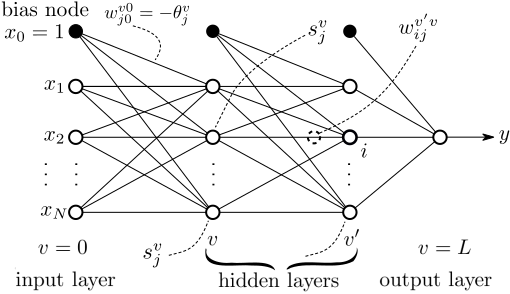
\includegraphics[height=5cm]{img/section1_fig14_fc}
    \mode<article>{
    \caption{MLP with fully connected layers}
    }
    \label{fig:mlp_fc}
    \end{figure}
    
\notesonly{Recall that the purpose of the Backpropagation algorithm is to compute the gradients. Therefore, the task is to obtain an expression for computing }\slidesonly{compute} the gradients for all weights and biases in this network:\\

\pause

\question{What is the general procedure for the Backpropagation algorithm?}

\mode<article>{
\pause
- The procedure is:
\begin{enumerate}
 \item Forward pass: forward propagation of neuron activities and obtain the network's response,
 \item Backward pass: backpropagation of ``local errors''
\end{enumerate}
}
\end{frame}

\begin{frame}
    \mode<presentation>{
    \placeimage{7.4}{1}{img/section1_fig14_fc}{width=6.7cm}
    \begin{textblock}{4}(0.5,2)
    \begin{equation}
    \boxed{
    \only<-8>{
    \frametitle{The forward pass}
        {\color{darkgreen}h_i^{v'}}
        \,= \kern-2ex
        \smallsum{(\mu,k) \in P(v',\,i)}{}
        \kern-2ex
        w_{ik}^{v'\mu}\; f_k^\mu\big( {\color{teal} h_k^\mu} \big)
    }
    \only<9->{
    \frametitle{The backward pass}
            {\color{red}\delta_i^{v'}}
            =
            [f_i^{v'}]'({\color{darkgreen}h_i^{v'}}) 
            \kern-3ex\sum_{(v''\hspace{-1mm},\,k) \in C(v',\,i)}\kern-3ex
            {\color{red}\delta_k^{v''}} 
            {w}_{ki}^{v'' v'}
            }
            }
    \end{equation}
    \end{textblock}
    \vspace{2cm}
    }
    
    Compute $h^{v}_{i}$ for $v = 0,\ldots,L$:
    \begin{itemize}
    \only<1,2,15,16>{
        \item $v=0$ (input layer):\\ \slidesonly{\vspace{-3mm}}
        \begin{flalign}
            h^{0}_{j} &=
            \only<1>{&&}
            \only<2,15,16>{
                              x_{j}\;,   & j=1,\ldots,N&&\\
                h^{0}_{0}  &= 1          & (\text{bias node})\\
                \vec h^{0} &= \vec x     & (\text{bias included})\\
                f^0_{j}(h) :\kern-0.5ex&= h \qquad\Rightarrow\; \vec f^0(\vec h) = \vec x
                & \text{ (identity function)}\\
            }
            \only<15,16>{{\color{red}\delta^{0}_{j}}
             &=}
             \only<16>{\text{Not applicable to observed input}}
        \end{flalign}
    }
    \only<3,4,13,14>{
        \item $v=1$ (1\textsuperscript{st} hidden layer, $N^{(1)} \text{ nodes}$):\\ \slidesonly{\vspace{-5mm}}
        \begin{flalign}
        h^{1}_{j} &= 
        \only<3>{&&}
        \only<4,13,14>{
            \smallsum{k=0}{N} w_{jk}^{10}\;  f_k^0\big( {h_k^0} \big) = (\vec w_{j}^{10})^{\top} \vec h^0 & (\text{bias included})&&\\
            \vec h^{1} &= (\vec W^{10})^{\top} \vec h^0 &(\text{biases included})\\
            f^1_{j}(h) &= \text{e.g. }\tanh() & j=1,\ldots,N^{(1)}\\
        }
        \only<13,14>{
             {\color{red}\delta^{1}_{j}}
             &=
             \only<14>{\slidesonly{\scriptstyle}
                         %[f_i^{v'}]'({\color{darkgreen}h_i^{v'}}) 
            %\sum_{(v''\hspace{-1mm},\,k) \in C(v',\,i)}
            %{\color{red}\delta_k^{v''}} 
            %{w}_{ki}^{v'' v'}
            [f_j^{1}]'({\color{darkgreen}h_j^{1}}) 
            \kern-.5ex\sum_{k=0}^{N^{(2)}}\kern-.5ex
            {\color{red}\delta_k^{2}} \,
            {w}_{kj}^{21}
            = 
            [f_j^{1}]'({\color{darkgreen}h_j^{1}})\,
            {\color{red} (\vec \delta^{2})^{\top}}
            \vec {w}_{j}^{21}\\
             {\color{red} \vec \delta^{1}}
             &=
            {\slidesonly{\scriptstyle}
            [\vec f^{1}]'({\color{darkgreen}h^{1}})\,
            ({\color{red} (\vec \delta^{2})^{\top}}
            \vec {W}^{21})^{\top}
            ([\vec f^{1}]'({\color{darkgreen}h^{1}}))^{\top}
            ({\color{red} (\vec \delta^{2})^{\top}}
            \vec {W}^{21})?%TODO
            }
             }
        }
        \end{flalign}
    }
    \only<5,6,11,12>{
        \item $v=2$ (2\textsuperscript{nd} hidden layer, $N^{(2)} \text{ nodes}$):\\ \slidesonly{\vspace{-3mm}}
        \begin{flalign}
        h^{2}_{i} &=
        \only<5>{&&}
        \only<6,11,12>{
            \smallsum{j=0}{N^{(1)}} w_{ij}^{21}\;  f_j^1\big( {h_j^1} \big) = (\vec w_{i}^{21})^{\top} \vec f^{1}(\vec h^1) &(\text{bias included})&&\\
            \vec h^{2} &= (\vec W^{21})^{\top} \vec f^{1}(\vec h^1) &(\text{biases included})\\
            f^2_{i}(h) &= \text{e.g. }\tanh() & i=1,\ldots,N^{(2)}\\
        }
        \only<11,12>{
             {\color{red}\delta^{2}_{i}}
             &=
            \only<12>{
                [f_i^{2}]'({\color{darkgreen}h_i^{2}})
                {\color{red}\delta_1^{L}} 
                {w}_{1i}^{L2}\\
             {\color{red} \vec \delta^{2}} &=\; (\vec w^{L2})^{\top}[\vec f^{2}]'(\vec {\color{darkgreen}h^{2}})
            }
        }
        \end{flalign}
        }
    \only<7,8,9,10>{
        \item $v=L$ (output layer):\\ \slidesonly{\vspace{-4mm}}
        \begin{flalign}
        h^{L}_{1} &=
        \only<7>{&&}
        \only<8,9,10>{
            \smallsum{i=0}{N^{(2)}} w_{1i}^{L2}\;  f_i^1\big( {h_i^1} \big) = (\vec w_{1}^{21})^{\top} \vec f^{2}(\vec h^2) &(\text{bias included})&&\\
            y(\vec x; \vec w) &= f^L_{1}(h^{L}_{1})&&\\
            f^L_{1}(h) &= \text{e.g. logistic function (sigmoid)}\\
        }
        \only<9,10>{
            {\color{red}\delta^{L}_{1}}  &= \frac{\partial y(\vec{x}; \vec{w})} {{\color{blue}\partial h_1^{L}}} =
            \only<10>{
                [f_1^{L}]'({\color{blue} h_1^{L}})
            }
        }
        \end{flalign}
    }
    \end{itemize}
    
\end{frame}

\newpage

\subsection{Summary of the Backpropagation for gradient descent}

\begin{frame} \frametitle{\subsecname}
    \mode<presentation>{
	\only<1>{
		\placeimage{10.75}{5.5}{img/MLP_forward.pdf}{width=3.75cm}
		\placeimage{10.75}{8.7}{img/MLP_backward.pdf}{width=3.75cm}
	}}
     \only<2> {
		%\begin{minipage}{4}(11.5,5)
			%{\color{blue}
				%\footnotesize
				%\begin{center}
					%computational and 
					%memory complexity \\[2mm]
					%{\color{red}
						%$\mathcal{O}(n)$, %\quad
					%} \\[2mm]
					%$n$: number of weights
					%i.e.~{\em linear} in the 
					%number of weights
				%\end{center}
			%}
		%\end{minipage}
	}
	
	%\begin{algorithm}[H] 
		%\scriptsize
		\footnotesize
		\DontPrintSemicolon
		initialization of weights and thresholds \\
        
		\While{stopping criterion not met}{
			$\text{gradient}_{ij}^{v'v} := 0 
					\,, \quad \forall w_{ij}^{v'v}$ \\
                    
			\For{$\alpha \in \{1,\ldots,p\}$}{
				${\color{forward}h_i^0} 
					:= x_i^{(\alpha)} \,, \quad \forall i$ 
				\qquad\qquad // {\color{forward}forward propagation}\\
                
				\For{$v' \in \{1,\ldots,L\}$}{
					%~ ${\color{forward} h_i^{v'}} 
						%~ := \sum\limits_{\scriptscriptstyle
							%~ (v',i) \in C(v,j)} w_{ij}^{v'v} 
							${\color{forward}h_i^{v'}}
		   			\;\;=\;\; \kern-2ex\smallsum{(\mu,k) \in P(v',i)}{} \kern-2ex
	   			w_{ik}^{v'\mu}\;  \underbrace{f_k^\mu\big( {\color{forward} h_k^\mu} \big) 
								%~ \underbrace{f_j^v({\color{forward} h_j^{v}})
								}_{\kern-2exx_k^{(\alpha)} \;\text{if}\; 
									v'=1\kern-2ex } \,,
							\quad \forall i$
					\vspace{-1.5mm}
				}
				${\color{backward} \delta_1^L} 
					:= [f_1^L]'({\color{forward}h_1^L}) $%\,, \quad \forall i$ 
				\qquad // {\color{backward}backward propagation}\\
                
				\For{$v' \in \{L-1,\ldots,1\}$} {
					${\color{backward}\delta_i^{v'}} 
						:= [f_{i}^{v'}]'({\color{forward}h_i^{v'}}) 
						\kern-1ex\sum\limits_{(\mu,k) \in C(v',i)}\kern-1ex
						{\color{backward} \delta_k^{\mu}} 
						\, w_{ki}^{\mu v'} \;,
						\quad \forall i$
					\vspace{-2.5mm}
				}
				$\text{gradient}_{ij}^{v'v} := \text{gradient}_{ij}^{v'v}
						+ \frac{\partial e^{(\alpha)}}{\partial y(\vec x; \vec w)}
						 \, {\color{backward}\delta_i^{v'}} 
						 \, f_j^v({\color{forward}h_j^v})
						 \,, \quad \forall w_{ij}^{v'v}$
				\hspace{11mm} // sum
			}
			\notesonly{ // gradient descent step:\\
            
            }
			$\text{gradient}_{ij}^{v'v} := \frac{1}{p} \text{gradient}_{ij}^{v'v}$\\
			% $w_{ij}^{v'v} := w_{ij}^{v'v} - \frac{\hat \eta}{p}
			 $w_{ij}^{v'v} := w_{ij}^{v'v} - \eta
					\, \text{gradient}_{ij}^{v'v} 
					\,, \quad \forall w_{ij}^{v'v}	$
			\slidesonly{\hspace{15mm} // gradient descent step}
					\vspace{-1.5mm}
		}
		%\caption{Backpropagation in feedforward networks}
	%\end{algorithm}
\end{frame}


